%! Author = Juniell
%! Date = 10.05.2021

% Preamble
\documentclass[a4paper, 14pt]{extarticle}

% Packages
\usepackage[T2A]{fontenc}
\usepackage{natbib}
\usepackage{graphicx}
\usepackage[english, russian]{babel}
\usepackage{fontspec}
\usepackage{amsmath}
\usepackage{amsfonts}
\usepackage{amssymb}
\usepackage{amsthm}
\usepackage{mathtools}
\usepackage{mathrsfs}
\usepackage{fullpage}
\usepackage{ulem}
\usepackage{setspace}
\usepackage{listings}
\usepackage{indentfirst}
\usepackage[left=2cm,right=1.5cm,top=2cm,bottom=2cm]{geometry}
\usepackage{xcolor}
\usepackage{float}
\usepackage{csquotes}
\usepackage{hyperref}
\usepackage{graphics}

\definecolor{urlcolor}{HTML}{0000FF} % цвет ссылок
\definecolor{linkcolor}{HTML}{000000} % цвет гиперссылок
\hypersetup{pdfstartview=FitH, linkcolor=linkcolor, urlcolor=urlcolor, colorlinks=true}

\setmainfont{Times New Roman}
\setlength{\parindent}{5ex}
\setlength{\parskip}{1em}
\renewcommand{\baselinestretch}{1}

\graphicspath{{resources/Images}}

\definecolor{buzzlightyear}{HTML}{8757A5}
\definecolor{grass}{HTML}{738D06}
\definecolor{literal}{HTML}{F18A2B}
\definecolor{commentcolor}{HTML}{8E908B}

\lstdefinestyle{habrstyle}{
    backgroundcolor=\color{white},
    commentstyle=\color{commentcolor},
    keywordstyle=\bfseries\color{buzzlightyear},
    numberstyle=\tiny\color{commentcolor},
    stringstyle=\color{grass},
    basicstyle=\ttfamily\footnotesize,
    breakatwhitespace=false,
    breaklines=true,
    captionpos=b,
    keepspaces=true,
    numbers=left,
    numbersep=5pt,
    showspaces=false,
    showstringspaces=false,
    showtabs=false,
    tabsize=4,
    language=Python
}

\lstset{style=habrstyle}


% Document
\begin{document}
% Титульный лист
    \begin{center}
        \begin{center}
            \hfill \break
            \normalsize{Санкт-Петербургский государственный политехнический}\\
            \normalsize{университет Петра Великого}\\
            \hfill \break
            \normalsize{\textbf{Высшая школа интеллектуальных систем и}}\\
            \normalsize{\textbf{суперкомпьютерных технологий}}\\
            \hfill \break
            \hfill \break
            \hfill \break
            \hfill \break
            \hfill \break
            \normalsize{Отчёт по лабораторной работе №6}\\
            \normalsize{Дисциплина: Телекоммуникационные технологии}\\
            \normalsize{Тема: Дискретное косинусное преобразование}\\
        \end{center}
        \hfill \break
        \hfill \break
        \hfill \break
        \hfill \break
        \hfill \break
        \hfill \break
        \hfill \break
        \hfill \break
        \hfill \break
        \hfill \break
        \begin{tabbing}
            Выполнил студент гр. 3530901/80201 \`В.А. Пучкина\\
            \\
            Преподаватель: \`Н.В. Богач\\
        \end{tabbing}
        \hfill \break
        \hfill \break
        \hfill \break
        \hfill \break
        \begin{center}
            Санкт-Петербург\\
            2021
        \end{center}
        \thispagestyle{empty}
    \end{center}

% Оглавление
    \newpage
    \tableofcontents

% Список иллюстраций
    \newpage
    \listoffigures

% Список листингов
    \newpage
    \lstlistoflistings

% ---------------------------------------------- Упражнение 6.1 ----------------------------------------------
    \newpage
    \section{Упражнение 6.1}
    \label{sec:task1}

    В этом упражнении необходимо провести следующую проверку: запускать функции \texttt{analyze} и \texttt{analyze2} с разными массивами и
    засекать время работы, после чего вывести зависимость времени работы от размера массива на логарифмической шкале.
    То же самое необходимо проделать для \texttt{scipy.fftpack.dct}.

    Сначала создадим шумовой сигнал.

    \begin{lstlisting}[caption= Создание шумового сигнала., label={lst:task1_signal}]
signal = UncorrelatedGaussianNoise()
noise = signal.make_wave(duration=1, framerate=16384)   \end{lstlisting}

    Теперь определим необходимые функции:
    \begin{itemize}
        \item \texttt{plot\_bests} для отображения массива результата,
        \item \texttt{run\_speed\_test} для запуска теста,
        \item \texttt{analyze1},
        \item \texttt{analyze2}.
    \end{itemize}

    \begin{lstlisting}[caption= Функция \texttt{plot\_bests}., label={lst:task1_plot_bests}]
def plot_bests(ns, bests):
    plt.plot(ns, bests)
    decorate(xscale='log', yscale='log')

    x = numpy.log(ns)
    y = numpy.log(bests)
    t = linregress(x,y)
    slope = t[0]
    return slope    \end{lstlisting}

    \begin{lstlisting}[caption= Функция \texttt{run\_speed\_test}., label={lst:task1_run_speed_test}]
def run_speed_test(ns, func):
    results = []
    for N in ns:
        print(N)
        ts = (0.5 + numpy.arange(N)) / N
        freqs = (0.5 + numpy.arange(N)) / 2
        ys = noise.ys[:N]
        result = %timeit -r1 -o func(ys, freqs, ts)
        results.append(result)

    bests = [result.best for result in results]
    return bests    \end{lstlisting}

    \begin{lstlisting}[caption= Функция \texttt{analyze1}., label={lst:task1_analyze1}]
PI2 = numpy.pi * 2

def analyze1(ys, fs, ts):
    args = numpy.outer(ts, fs)
    M = numpy.cos(PI2 * args)
    amps = numpy.linalg.solve(M, ys)
    return amps     \end{lstlisting}

    \begin{lstlisting}[caption= Функция \texttt{analyze2}., label={lst:task1_analyze2}]
def analyze2(ys, fs, ts):
    args = numpy.outer(ts, fs)
    M = numpy.cos(PI2 * args)
    amps = numpy.dot(M, ys) / 2
    return amps     \end{lstlisting}

    Итак, подготовим данные для тестирования. Для чистоты эксперимента будем использовать одинаковые данные для всех
    тестируемых функций.

    \begin{lstlisting}[caption= Формирование тестовых данных., label={lst:task1_data}]
ns = 2 ** numpy.arange(7, 14)   \end{lstlisting}

    Теперь протестируем \texttt{analyze1}.

    \begin{lstlisting}[caption= Тестирование \texttt{analyze1}., label={lst:task1_test_analyze1}]
bests = run_speed_test(ns, analyze1)
plot_bests(ns, bests)   \end{lstlisting}

    \begin{figure}[h]
        \centering
        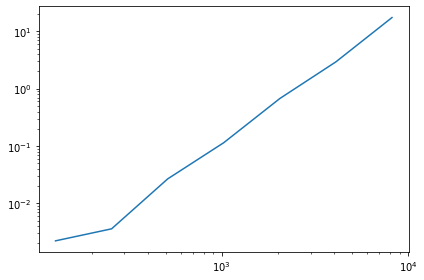
\includegraphics[width=0.8\linewidth]{resources/Images/task1_test_analyze1}
        \caption{Зависимость времени работы от размера (\texttt{analyze1}).}
        \label{fig:task1_test_analyze1}
    \end{figure}

    Рассчитанный наклон составил примерно 2.2, что не соответствует ожиданиям.
    Такой результат мог возникнуть из-за выборки в массиве.

    Протестируем \texttt{analyze2}.

    \begin{lstlisting}[caption= Тестирование \texttt{analyze1}., label={lst:task1_test_analyze2}]
bests2 = run_speed_test(ns, analyze2)
plot_bests(ns, bests2)  \end{lstlisting}

    \begin{figure}[h]
        \centering
        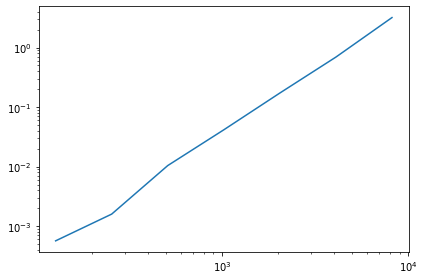
\includegraphics[width=0.8\linewidth]{resources/Images/task1_test_analyze2}
        \caption{Зависимость времени работы от размера (\texttt{analyze2}).}
        \label{fig:task1_test_analyze2}
    \end{figure}

    Для \texttt{analyze2} рассчитанный наклон составил примерно 2.1, что совпало с ожиданиями.

    И наконец, протестируем \texttt{scipy\_dct}.

    \begin{lstlisting}[caption= Функция \texttt{scipy\_dct}., label={lst:task1_test_scipy_dct}]
bests2 = run_speed_test(ns, analyze2)
plot_bests(ns, bests2)  \end{lstlisting}

    Эта реализация работает ещё быстрее. По зависимости времени работы от размера (Рис.\ref{fig:task1_test_scipy_dct}) видно,
    что зависимости нелинейна (график изогнут). Это означает, что либо мы еще не видели асимптотическое поведение,
    либо асимптотическое поведение не является простым показателем $n$. Её время выполнения пропорционально
    $n log n$.

    \begin{figure}[H]
        \centering
        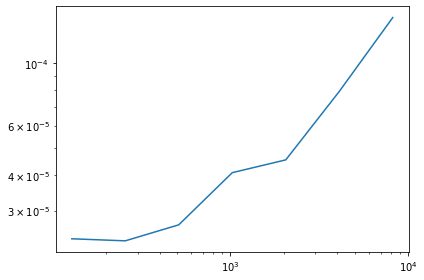
\includegraphics[width=0.7\linewidth]{resources/Images/task1_test_scipy_dct}
        \caption{Зависимость времени работы от размера (\texttt{scipy\_dct}).}
        \label{fig:task1_test_scipy_dct}
    \end{figure}

    Теперь сравним все полученные результаты, для этого выведем их не один график.

    \begin{lstlisting}[caption= Сравнение полученных результатов., label={lst:task1_test_all}]
plt.plot(ns, bests, label='analyze1')
plt.plot(ns, bests2, label='analyze2')
plt.plot(ns, bests3, label='fftpack.dct')
decorate(xlabel='Wave length (N)', ylabel='Time (s)', xscale='log', yscale='log')   \end{lstlisting}

    \begin{figure}[h]
        \centering
        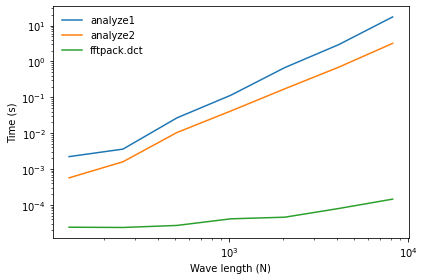
\includegraphics[width=0.7\linewidth]{resources/Images/task1_test_all}
        \caption{Зависимости времени работы от размера массива для разных функций.}
        \label{fig:task1_test_all}
    \end{figure}

    Таким образом, из полученного графика (Рис.\ref{fig:task1_test_all}) видно, что \texttt{scipy\_dct} является самой
    быстрой реализацией.

    В ходе выполнения данного упражнения были получены зависимости времени работы от размера массива для функций
    \texttt{analyze1}, \texttt{analyze2} и \texttt{scipy\_dct}. Также был получен общий график зависимостей. По полученным
    результатам был сделан вывод, что \texttt{scipy\_dct} является самой быстрой реализацией.

    \newpage

    % ---------------------------------------------- Упражнение 6.2 ----------------------------------------------
    \section{Упражнение 6.2}
    \label{sec:task2}

    В этом упражнении необходимо реализовать алгоритм для сжатия с помощью ДКП. После чего применить полученный алгоритм
    на записи музыки или речи.

    Итак, для проверки будем использовать запись гитары, скаченную \href{https://freesound.org/people/SeryLis/sounds/181425/}{отсюда}.

    \begin{lstlisting}[caption= Чтение файла и получение \texttt{wave}., label={lst:task2_wave}]
guitar_wave = read_wave('resources/Sounds/task2_serylis_guitar_chord.wav')
guitar_wave.make_audio()    \end{lstlisting}

    \begin{lstlisting}[caption= Выбор сегмента., label={lst:task2_segment}]
guitar_segment = guitar_wave.segment(start=0.7, duration=0.5)
guitar_segment.normalize()
guitar_segment.make_audio() \end{lstlisting}

    Теперь получим ДКП сегмента.

    \begin{lstlisting}[caption= Получение ДКП., label={lst:task2_dct}]
guitar_dct = guitar_segment.make_dct()
guitar_dct.plot(high=1500)
decorate(xlabel='Frequency (Hz)', ylabel='DCT')     \end{lstlisting}

    \begin{figure}[h]
        \centering
        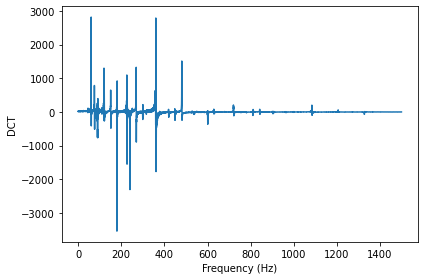
\includegraphics[width=0.8\linewidth]{resources/Images/task2_dct}
        \caption{ДКП сегмента.}
        \label{fig:task2_dct}
    \end{figure}

    Теперь реализуем алгоритм сжатия с помощью ДКП.

    \begin{lstlisting}[caption= Функция \texttt{compress} для сжатия., label={lst:task2_fun}]
def compress(dct, thresh=1):
    count = 0
    for i, amp in enumerate(dct.amps):
        if numpy.abs(amp) < thresh:
            dct.hs[i] = 0
            count += 1

    n = len(dct.amps)
    print(count, n, 100 * count / n, sep='\t')  \end{lstlisting}

    Применим функцию \texttt{compress} на нашем сегменте.

    \begin{lstlisting}[caption= Сжатие сегмента., label={lst:task2_dct_compress}]
compress(guitar_dct, thresh=10)
guitar_dct.plot(high=1500)
guitar_segment2 = guitar_dct.make_wave()
guitar_segment2.make_audio()    \end{lstlisting}

    \begin{figure}[h]
        \centering
        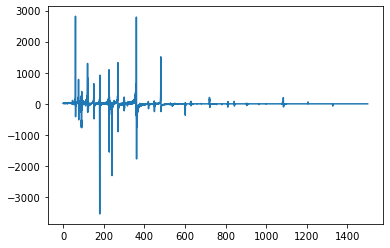
\includegraphics[width=0.8\linewidth]{resources/Images/task2_dct_compress}
        \caption{ДКП сжатого сегмента.}
        \label{fig:task2_dct_compress}
    \end{figure}

    При сравнении оригинального сегмента с полученным разница не слышима, несмотря на то что было удалено около 95\%
    гармоник.

    Теперь реализуем функцию для сжатия большого сегмента. Она аналогична \texttt{wave.make\_spectrogram}, только в ней
    используется ДКП.

    \begin{lstlisting}[caption= Функция \texttt{make\_dct\_spectrogram} для сжатия \texttt{wave}., label={lst:task2_fun2}]
def make_dct_spectrogram(wave, seg_length):
    window = numpy.hamming(seg_length)
    i, j = 0, seg_length
    step = seg_length // 2
    spec_map = {}

    while j < len(wave.ys):
        segment = wave.slice(i, j)
        segment.window(window)

        t = (segment.start + segment.end) / 2
        spec_map[t] = segment.make_dct()

        i += step
        j += step
    return Spectrogram(spec_map, seg_length)    \end{lstlisting}

    Используем полученную функцию на \texttt{wave} всей записи.

    \begin{lstlisting}[caption= Сжатие \texttt{wave} всей записи., label={lst:task2_fun2}]
guitar_spectrogram = make_dct_spectrogram(guitar_wave, seg_length=1024)
for t, dct in sorted(guitar_spectrogram.spec_map.items()):
    compress(dct, thresh=0.2)   \end{lstlisting}

    Прослушаем результат.

    \begin{lstlisting}[caption= Получение аудио результата., label={lst:task2_fun2}]
guitar_wave2 = guitar_spectrogram.make_wave()
guitar_wave2.make_audio()   \end{lstlisting}

    При сравнении полученного аудио с оригинальным разница не слышна, хотя на разных сегментах сжатие составляло от 50
    до 99\%.

    В ходе выполнения данного упражнения был реализован алгоритм для сжатия с помощью ДКП.
    Затем полученный алгоритм был использован на сегменте записи аккорда гитары. Несмотря на то что компрессия составила
    около 95\%, звучание не изменилось. Затем был использован алгоритм для сжатия \texttt{wave}.
    Компрессия на разных сегментах составляла от 50 до 99\%, но звук по прежнему воспринимается так же.

    \newpage

    % ---------------------------------------------- Упражнение 6.3 ----------------------------------------------
    \section{Упражнение 6.3}
    \label{sec:task3}

    В данном упражнении необходимо изучить файл \texttt{phase.ipnyb}, в котором исследуется влияние фазы на восприятие
    звука. После изучения примеров следует выбрать другой сегмент звука и повторить эксперименты.

    Итак, сначала определим необходимые функции, которые используются в файле \texttt{phase.ipnyb}.

    \begin{lstlisting}[caption= Функция \texttt{plot\_angle}., label={lst:task3_plot_angle}]
def plot_angle(spectrum, thresh=1):
    angles = spectrum.angles
    angles[spectrum.amps < thresh] = numpy.nan
    plt.plot(spectrum.fs, angles, 'x')
    decorate(xlabel='Frequency (Hz)', ylabel='Phase (radian)')  \end{lstlisting}

    \begin{lstlisting}[caption= Функция \texttt{plot\_three}., label={lst:task3_plot_three}]
def plot_three(spectrum, thresh=1):
    plt.figure(figsize=(10, 4))
    plt.subplot(1,3,1)
    spectrum.plot()
    plt.subplot(1,3,2)
    plot_angle(spectrum, thresh=thresh)
    plt.subplot(1,3,3)
    wave = spectrum.make_wave()
    wave.unbias()
    wave.normalize()
    wave.segment(duration=0.01).plot()
    display(wave.make_audio())      \end{lstlisting}

    \begin{lstlisting}[caption= Функция \texttt{zero\_angle}., label={lst:task3_zero_angle}]
def zero_angle(spectrum):
    res = spectrum.copy()
    res.hs = res.amps
    return res  \end{lstlisting}

    \begin{lstlisting}[caption= Функция \texttt{rotate\_angle}., label={lst:task3_rotate_angle}]
def rotate_angle(spectrum, offset):
    res = spectrum.copy()
    res.hs *= numpy.exp(1j * offset)
    return res      \end{lstlisting}

    \begin{lstlisting}[caption= Функция \texttt{random\_angle}., label={lst:task3_random_angle}]
def random_angle(spectrum):
    res = spectrum.copy()
    angles = numpy.random.uniform(0, PI2, len(spectrum))
    res.hs *= numpy.exp(1j * angles)
    return res      \end{lstlisting}

    Теперь считаем файл и выберем сегмент, отличный от использующегося в примере.

    \begin{lstlisting}[caption= Чтение файла., label={lst:task3_read}]
oboe_wave = read_wave('resources/Sounds/task3_thirsk_120_oboe.wav')
oboe_wave.make_audio()  \end{lstlisting}

    \begin{lstlisting}[caption= Выбор сегмента., label={lst:task3_segment}]
oboe_segment = oboe_wave.segment(start=2.1, duration=1)
oboe_segment.make_audio()
    \end{lstlisting}

    Используем на этом сегменте \texttt{plot\_three} для получения спектра, угловой части спектра и \texttt{wave}.

    \begin{lstlisting}[caption= Применение \texttt{plot\_three} к оригинальному сегменту., label={lst:task3_three}]
oboe_spectrum = oboe_segment.make_spectrum()
plot_three(oboe_spectrum, thresh=50)    \end{lstlisting}

    \begin{figure}[h]
        \centering
        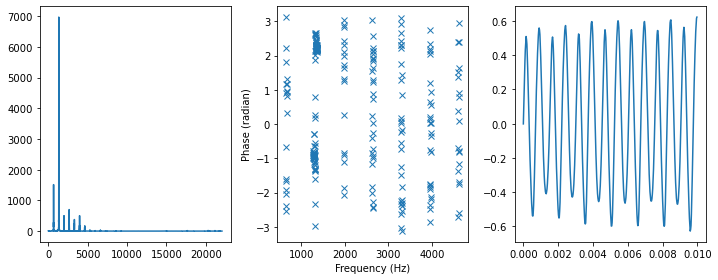
\includegraphics[width=0.8\linewidth]{resources/Images/task3_three}
        \caption{Спектр, фаза и \texttt{wave} оригинального сегмента.}
        \label{fig:task3_three}
    \end{figure}

    Теперь установим углы на нуль.

    \begin{lstlisting}[caption= Применение \texttt{plot\_three} к сегменту с нулевыми углами., label={lst:task3_three_zero}]
oboe_spectrum2 = zero_angle(oboe_spectrum)
plot_three(oboe_spectrum2)  \end{lstlisting}

    \begin{figure}[h]
        \centering
        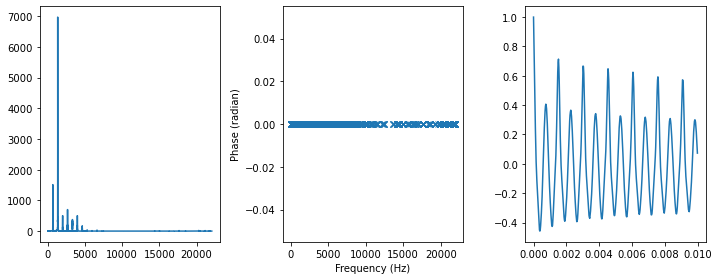
\includegraphics[width=0.8\linewidth]{resources/Images/task3_three_zero}
        \caption{Спектр, фаза и \texttt{wave} сегмента с нулевыми углами.}
        \label{fig:task3_three_zero}
    \end{figure}

    Можно заметить, что спектр не изменился, а вот форма \texttt{wave} изменилась.
    Изменение фазовой структуры создаёт эффект <<звона>>, когда громкость меняется со временем.

    Теперь повернём углы на 1 радиану.

    \begin{lstlisting}[caption= Применение \texttt{plot\_three} к сегменту с повёрнутыми углами., label={lst:task3_three_rotate}]
oboe_spectrum3 = rotate_angle(oboe_spectrum, 1)
plot_three(oboe_spectrum3)  \end{lstlisting}

    \begin{figure}[h]
        \centering
        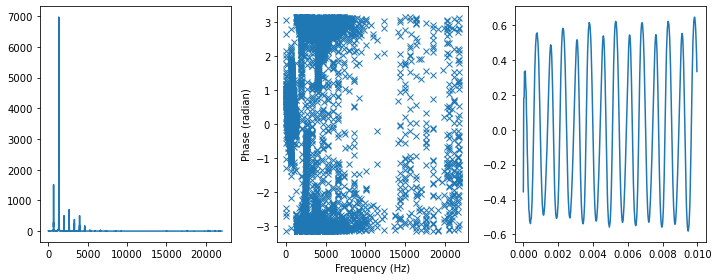
\includegraphics[width=0.8\linewidth]{resources/Images/task3_three_rotate}
        \caption{Спектр, фаза и \texttt{wave} сегмента с повёрнутыми углами.}
        \label{fig:task3_three_rotate}
    \end{figure}

    Вращение углов не вызывает эффекта <<звона>>.

    Теперь установим ля углов рандомные значения.

    \begin{lstlisting}[caption= Применение \texttt{plot\_three} к сегменту с рандомными углами., label={lst:task3_three_random}]
oboe_spectrum4 = random_angle(oboe_spectrum)
plot_three(oboe_spectrum4)
    \end{lstlisting}

    \begin{figure}[h]
        \centering
        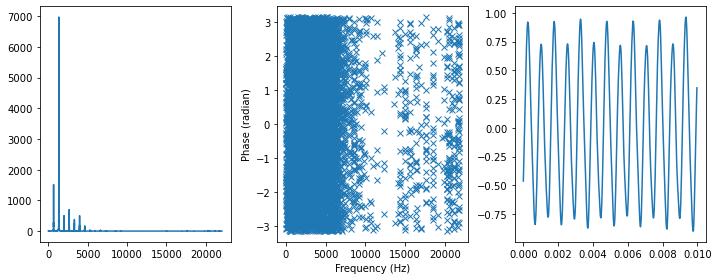
\includegraphics[width=0.8\linewidth]{resources/Images/task3_three_random}
        \caption{Спектр, фаза и \texttt{wave} сегмента с рандомными углами.}
        \label{fig:task3_three_random}
    \end{figure}

    В данном случае рандомные значения углов вызывают небольшой эффект <<звона>>, звук становится более сухим.


    В ходе выполнения данного упражнения исследовалось влияние фазы на восприятие звука. Для этого были изучены примеры,
    представленные в файле \texttt{phase.ipnyb}. После чего был выбран другой сегмент и проведён повторный эксперимент.
    Был сделан вывод, что для звуков с простой гармонической структурой изменения фазовой структуры не заметны на слух.
    Возможным исключением могут быть звуки с низкой амплитудой на основной частоте.

    \newpage

% ---------------------------------------------- Выводы ----------------------------------------------
    \section{Выводы}
    \label{sec:conclusions}

    В ходе данной лабораторной работы было изучено дискретное косинусное преобразование, были получены навыки по работе
    с ним. Кроме того, был написан и протестирован алгоритм для сжатия записи. Также было исследовано влияние фазы на
    восприятие звука с помощью анализа различных звуков и сегментов.

\end{document}